\section{Visual Perception Pipeline and Diagnostic Clip Study}

MANAR includes a C++ \texttt{Yolo11nDetector} wrapper and Python/C++ evaluation harnesses using ONNX Runtime~\cite{onnxruntime2019} and OpenCV. The detector produces instantaneous person-class events; tracking, identity persistence, geolocation, and rescue confirmation are deliberately outside this layer:
\begin{equation}
\mathbf{y}_k = \{\mathcal{B}_i,c_i\}_{i=1}^{M_k}, \qquad c_i \ge c_{\mathrm{th}}=0.50.
\end{equation}

\subsection{Tensor Contract and Export Reproducibility}

Each frame $I\in\mathbb{R}^{H\times W\times3}$ is resized with aspect-ratio-preserving letterboxing to $640\times640$, converted from BGR to RGB, normalized to $[0,1]$, and arranged as a \texttt{float32} NCHW tensor. The committed YOLO11n graph has input shape $[1,3,640,640]$ and output shape $[1,84,8400]$. Channels 0--3 encode $[c_x,c_y,w,h]$ and channels 4--83 encode COCO class scores. Person candidates are mapped through the inverse letterbox transformation and filtered with host-side non-maximum suppression at $\mathrm{IoU}_{\mathrm{NMS}}=0.45$.

The static graph was exported with the following recorded command:
\begin{lstlisting}[language=bash]
yolo export model=yolo11n.pt format=onnx imgsz=640 \
  dynamic=False opset=19
\end{lstlisting}
The artifact size is 10,720,228 bytes (10.22 MB), and its recorded SHA-256 suffix is \texttt{...00804cc5c1}. Future releases should publish the complete hash and the exact upstream checkpoint identifier in a machine-readable manifest.

\subsection{Corpus and Protocol}

The local corpus contains 26 clips under \texttt{assets/Videos/Training videos/}. Direct metadata inspection gives 240 frames per clip, 24 frames/s, and $1280\times720$ pixels, for 6,240 frames total. Eleven clips are designated negative by filename (\texttt{No Target} or \texttt{False Positive}), contributing 2,640 frames; 15 are designated positive (clear, moving, multiple-person, or partially concealed), contributing 3,600 frames. The filenames label RGB, infrared/low-light IR, and thermal conditions. Because the repository does not preserve capture-device, spectral-band, calibration, or transformation provenance, this paper calls the corpus \emph{multi-condition}, not a calibrated multispectral dataset.

YOLO11n and D-FINE-N~\cite{peng2024dfine} are evaluated zero-shot with batch size 1, a $640\times640$ model input, person-class threshold 0.50, and the ONNX Runtime CPU execution provider. The committed \texttt{perception/vision/benchmarks/results.md} stores one mean model-session latency and total event count for each model--clip pair. It does not store bounding-box ground truth, per-frame matches, raw timing samples, warm-up policy, repeated-run order, or a machine-readable hardware manifest.

For that reason, the reported measures are strictly:
\begin{itemize}
    \item \textbf{model-session latency:} the recorded mean time around the ONNX session call for each clip;
    \item \textbf{detection event:} one post-threshold person box emitted on one frame; repeated boxes on the same person count repeatedly;
    \item \textbf{positive-scenario coverage:} the fraction of the 15 positive-designated clips with at least one event; and
    \item \textbf{negative-designated events:} emitted events on the 11 clips designated as containing no person target.
\end{itemize}
These measures are not average precision, precision, recall, F1, unique-person count, or tracking accuracy.

\begin{table}[t]
\caption{Diagnostic 26-Clip Zero-Shot Comparison}
\label{tab:cv_benchmark_summary}
\centering
\footnotesize
\begin{tabularx}{\columnwidth}{@{}Xrr@{}}
\toprule
\textbf{Recorded measure} & \textbf{D-FINE-N} & \textbf{YOLO11n} \\
\midrule
Clip means available & 26 & 26 \\
Session latency, mean $\pm$ SD & $50.53\pm3.15$ ms & $29.25\pm0.85$ ms \\
Reciprocal session rate & 19.79 s$^{-1}$ & 34.19 s$^{-1}$ \\
Positive clips with $\ge1$ event & $6/15$ (40\%) & $12/15$ (80\%) \\
Events on positive clips & 892 & 1,497 \\
Events on negative clips & 0 & 0 \\
Model file size & 14.55 MB & 10.22 MB \\
\bottomrule
\end{tabularx}
\end{table}

\begin{figure*}[t]
\centering
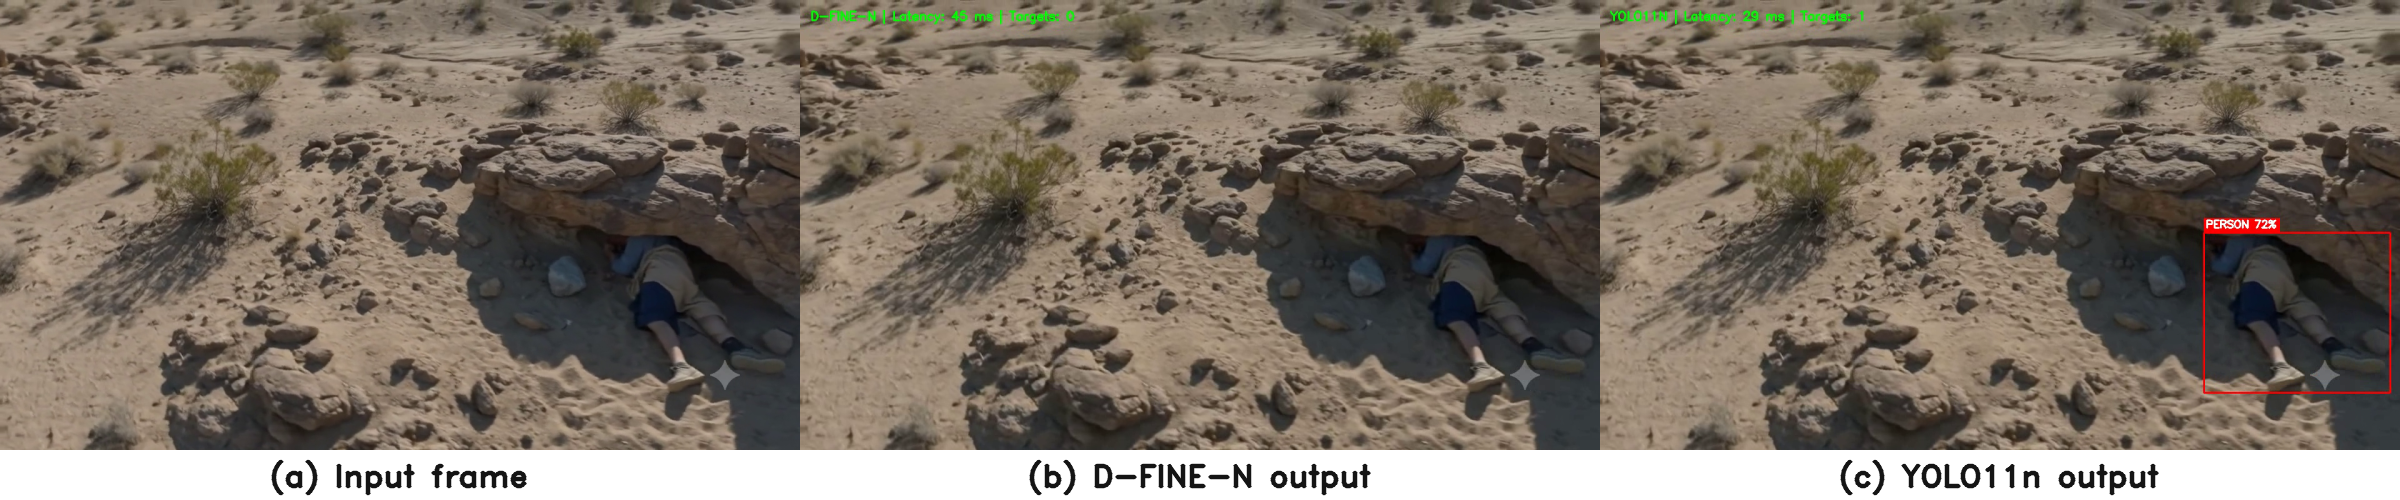
\includegraphics[width=\textwidth]{figures/detector_qualitative_comparison.png}
\caption{Frame-aligned qualitative example from the positive-designated \texttt{RGB Partially Concealed Rescuee} clip at frame 239. D-FINE-N emits no person event at the fixed threshold, whereas YOLO11n emits one. This selected example illustrates the event definition; without ground-truth boxes it is not an accuracy estimate.}
\label{fig:detector_qualitative_comparison}
\end{figure*}

\subsection{Observed Results}

Across the 26 recorded clip means, YOLO11n's model-session latency is 42.1\% lower than D-FINE-N's, a ratio of $1.73\times$. This is not an end-to-end throughput comparison: the graph boundaries differ and YOLO's host-side NMS lies outside the session timer. Decode, resize, normalization, postprocessing, rendering, and IPC must be timed separately before an onboard frame-rate claim is made.

YOLO11n produces at least one event in twice as many positive-designated clips (12 vs.\ 6) and 1.68$\times$ as many positive-clip events (1,497 vs.\ 892). Both produce zero events on the 11 negative-designated clips in this corpus. Event count is intentionally interpreted as sensitivity evidence only: it may reward duplicate detections, cannot identify missed ground-truth persons, and provides no localization score.

The result supports selecting YOLO11n as the present prototype's \emph{diagnostic} detector because it offers wider positive-scenario coverage and lower recorded session latency under the fixed protocol. It does not establish that dense convolutional detectors are generally superior to transformer detectors. Training data, confidence calibration, graph export, target scale, and postprocessing are confounded. A publication-level comparison requires matched threshold sweeps, ground-truth boxes, at least one additional baseline, and confidence intervals over repeated end-to-end runs.

\subsection{Planned Perception Extensions}

The next evidence milestones are (1) bounding-box annotation with target size and occlusion attributes, (2) held-out scenario/site splits, (3) threshold and input-resolution sensitivity studies, (4) slicing or tiling for small targets~\cite{akyon2022sahi}, and (5) multi-frame association using a tracker such as ByteTrack~\cite{zhang2022bytetrack}. Acoustic, radar, RF, and Mamba-based temporal fusion~\cite{gu2023mamba} remain planned and are not evaluated in this paper.
